\section{Two-Dimensional Systems}
\noindent\rule[\linienAbstand]{\linewidth}{\linienDickeDick}
We now consider the systmes for arbitrary $n \in \mathbb(N)$, i.e.
\begin{equation}
  \begin{split}
    \dot{x}_1 &= f_1(x_1, x_2,...,x_n)\\
    \dot{x}_2 &= f_2(x_1, x_2,...,x_n)\\
     &\;\;...\\
    \dot{x}_n &= f_n(x_1, x_2,...,x_n)
  \end{split}
\end{equation}
resp. in vector notation
\begin{equation}
  \dot{\mathbf{x}} = \mathbf{f}(\mathbf{x}) \;\;\; (\mathbf{x}\in\mathbb(R)^n)
\end{equation}



\textbf{Definitions}\\
A point $x^* \in \mathbb{R}^n$ is a \emph{fixed point} of the dynamical system $\dot{\mathbf{x}} =  \mathbf{f}(\mathbf{x})$, if
\begin{equation}
  \mathbf{f}(\mathbf{x^*}) = \mathbf{0}
\end{equation}
If $\mathbf{x^*}$ is a \emph{fixed point} of the dynamical system $\dot{\mathbf{x}} =  \mathbf{f}(\mathbf{x})$, then
\begin{equation}
   \mathbf{x}(t) =  \mathbf{x}^*
\end{equation}
is a constant solution.\\

A fixed point $x^* \in \mathbb{R}^n$ of the dynamical system $\dot{\mathbf{x}} =  \mathbf{f}(\mathbf{x})$, is
\begin{itemize}
  \item \emph{stable}, if the solution starting close to $x^*$ stays close to $x^*$ for all $t \geq 0$.
  \item \emph{asymptotically stable}, if the solution starting close to $x^*$ converge to $x^*$ for $t \rightarrow \infty$.
  \item \emph{unstable}, if the solution starts close to $x^*$ and diverging from $x^*$ for $t \rightarrow \infty$.
\end{itemize}

\subsection{Linear Systems}
\noindent\rule[\linienAbstand]{\linewidth}{\linienDicke}

Overview over the various types of fixed points and the corresponding geometry of the system near the fixed point:
\begin{figure}[H]
  \centering
  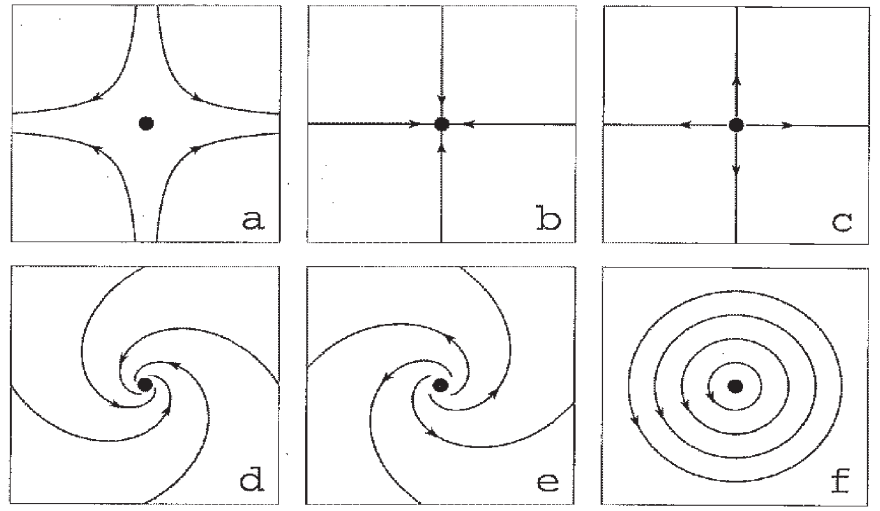
\includegraphics[width=.7\linewidth]{Pics/4.18.png}
\end{figure}

\begin{table}[H]
  \footnotesize
  \begin{tabular}{ll}
    a) saddle point    & e) unstable spiral\\
    b) stable node     & f) center/elliptic fixed point\\
    c) unstable node   & g) degenerate cases\\
    d) stable spiral   &
  \end{tabular}
\end{table}

A two-dimensional system can be characterized with the eigenvalues like so:
\begin{itemize}
  \item $\lambda_1 < 0, \lambda_2 < 0$: stable node
  \item $\lambda_1 > 0, \lambda_2 < 0$: saddle point
  \item $\lambda_1 > 0, \lambda_2 > 0$: usntable point
  \item $\lambda_1 = 0, \lambda_2 = 0$: non-isolated fixed point
  \item $\lambda_{1.2} \neq \mathbb{R}, \textup{Re}(\lambda_{1,2}) = 0$: center
  \item $\lambda_{1.2} \neq \mathbb{R}, \textup{Re}(\lambda_{1,2}) > 0$: unstable spiral
  \item $\lambda_{1.2} \neq \mathbb{R}, \textup{Re}(\lambda_{1,2}) < 0$: stable spiral
\end{itemize}

Alternativ characterization instead of with the eigenvalues $\lambda_1, \lambda_2$ with trace and determinant of A:
\begin{equation}
  \begin{split}
    \tau &= \textup{tr} = a_{11} + a_{22}\\
    \Delta &= \textup{det}(A) = a_{11}a_{22} - a_{12}a_{21}
  \end{split}
\end{equation}
Connection with the eigenvalues:
\begin{equation}
  \lambda_{1,2} = \frac{1}{2}\left(\tau \pm \sqrt{\tau^2 - 4\Delta}\right)
\end{equation}
and
\begin{equation}
  \Delta = \lambda_1 \lambda_2, \;\;\; \tau = \lambda_1 + \lambda_2
\end{equation}
% - $\Delta > 0$ for all stable/unstable spirals and nodes, $\Delta < 0$ for saddle points\\
% - In the case $\Delta > 0$, the stable resp. unstable cases can be distinguished by $\tau < 0$ resp. $\tau > 0$\\
% - The distinction between nodes and spirals depends on the sign of $\tau^2 - 4\Delta$\\
% - $\tau = 0$: center stable\\

\begin{figure}[H]
  \centering
  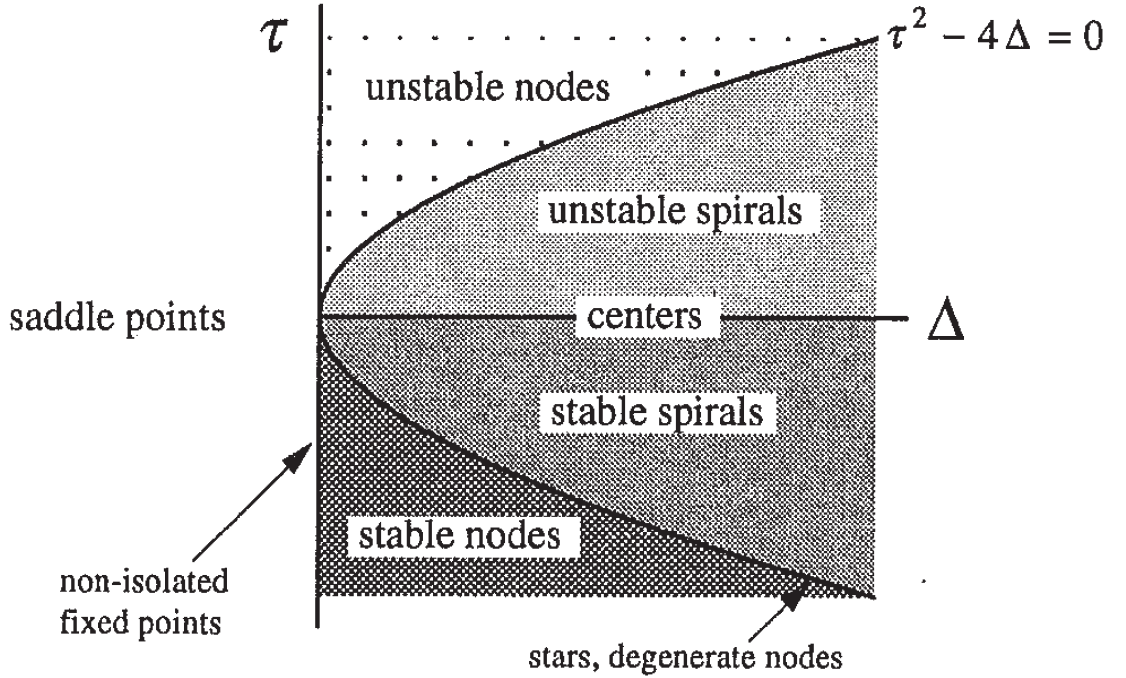
\includegraphics[width=.7\linewidth]{Pics/4.19.png}
\end{figure}

If one is only interested in the stability of $\textbf{x}^*$ (and not in a further classification into nodes,
spirals, etc.), the fixed point $\textbf{x}^* = 0$ of a dynamical system is
\begin{itemize}
  \item asymptotically stable, if
  \begin{equation}
    \textup{Re}(\lambda_i) < 0
  \end{equation}
  holds for all eigenvalues $\lambda_i$ of $A$

  \item stable, if
  \begin{equation}
    \textup{Re}(\lambda_i) \leq 0
  \end{equation}
  holds for all eigenvalues $\lambda_i$ of $A$

  \item usntable, if
  \begin{equation}
    \textup{Re}(\lambda_i) > 0
  \end{equation}
  holds for at least one eigenvalue $\lambda_i$ of $A$
\end{itemize}

\subsection{Nonlinear Systems}
\noindent\rule[\linienAbstand]{\linewidth}{\linienDicke}
The behaviour of nonlinear systems can be investigated by analyzing the corresponding linear system near the fixed point $(x_1^*, x_2^*)$ and by then classifying these fixpoints according to the scheme for fixed points of linear systems.


find fixpoints
calculate jacobi-matrix
insert fixpoitns and analyse matrix

Example:
\begin{equation}
  \begin{split}
    \dot{x} &= -x + x^3\\
    \dot{y} &= -2y
  \end{split}
\end{equation}
fixed points are:
\begin{equation}
  P_1 = (0, 0), \;\; P_2 = (1, 0), \;\; P_3 = (-1, 0).
\end{equation}
The Jacobi matrix of the system is
\begin{equation}
  A = \begin{vmatrix}
      -1+3x^2 & 0 \\
      0 & -2
  \end{vmatrix}
\end{equation}
The eigenvalues of $A$ are:
\begin{equation}
  P_1: \lambda_1 = -1, \lambda_2 = -2; \;\;\; P_2, P_3: \lambda_{1,2} = \pm 2
\end{equation}
Therefore $P_1$ is a stable node, and $P_2$ and $P_3$ are saddle points of the linearized system.

\subsection{Bifurications}
\noindent\rule[\linienAbstand]{\linewidth}{\linienDicke}
